\chapter{Manual de Usuario\label{extra:manual_de_usuario}}

Este manual pretende ser una guía en la instalación, configuración y uso de la interfaz web para la gestión de sondas de red de altas prestaciones.

\section{Instalación del Servicio Web FPGA\label{extra:manual:instalacionfpga}}

\subsection*{Requisitos}
El servidor que aloje el \gls{servicioweb} \gls{FPGA} debe cumplir los siguientes requisitos:
\begin{itemize}
  \item La \gls{FPGA} para capturar/reproducir tráfico debe estar conectada.
  \item El sistema operativo debe estar basado en una distribución \textit{Debian} \cite{debian} y tener una arquitectura de 64 bits.
  \item La opción por defecto en el gestor de arranque debe ser iniciar con la opción \textit{HugePages} activa.
  \item El usuario \textit{root} debe existir.
\end{itemize}

\subsection*{Instalación}
Para instalar el \gls{servicioweb} \gls{FPGA}, compruebe que se cumplan todos los requisitos y siga los siguientes pasos:
\begin{enumerate}
  \item Descargue el código fuente del repositorio del proyecto (\href{https://github.com/JSidrach/NetWatcher/archive/master.zip}{\footnotesize{github.com/JSidrach/NetWatcher}}). La instalación se realiza de forma remota, así que no es necesario descargárselo en el propio servidor, aunque sí en un entorno con terminal.
  \item Descomprima el archivo \textit{.zip}.
  \item Edite el archivo \texttt{./fpga-api/scripts/update\_server.sh}, estableciendo los parámetros \texttt{SERVER\_IP} y \texttt{SERVER\_PATH} como la dirección del servidor remoto que alojará el \gls{servicioweb} \gls{FPGA} y la ruta donde guardar el código, respectivamente.
  \item Sitúese en la carpeta \texttt{./fpga-api/}.
  \item Despliegue el servidor ejecutando el siguiente comando:
  
  \texttt{./scripts/update\_server.sh}
  \item Inicie sesión en el servidor remoto.
  \item Ponga en marcha el \gls{servicioweb} ejecutando el siguiente comando:

  \texttt{sudo service fpga-api start}
  \item Compruebe que el servidor está activo con el siguiente comando:

  \texttt{sudo service fpga-api status}
\end{enumerate}


\section{Configuración del Servicio Web FPGA\label{extra:manual:configfpga}}
Para configurar el \gls{servicioweb} \gls{FPGA}, inicie sesión en el servidor en el que se instaló este servicio. Los distintos parámetros de configuración vienen recogidos en el archivo \texttt{config.js}, dentro de la carpeta raíz del servicio (el contenido de la variable \texttt{SERVER\_PATH}, establecida en la instalación). Edite las distintas variables de este archivo (explicadas en la Tabla \ref{extra:manual:paramsfpga}) para configurar el servicio. No es necesario reiniciar el servicio para que los cambios en el archivo \texttt{config.js} se reflejen en el servidor.

\begin{table}
\centering
\begin{tabular}{|l|l|l|}
\hline
\rowcolor[HTML]{F5F5F5}
\textbf{Variable}   & \textbf{Tipo}    & \textbf{Descripción}                                           \\ \hline
BASE\_PREFIX        & Cadena de texto  & Prefijo base de la \gls{API}                                   \\ \hline
PORT                & Número entero    & Puerto del servicio                                            \\ \hline
MAX\_DELAY          & Número entero    & Retraso máximo entre el \textit{timestamp} de las              \\
                    &                  & peticiones y el \textit{timestamp} del servidor. Si            \\
                    &                  & es menor o igual que 0, no se descartará                       \\ 
                    &                  & ninguna petición basándose en el \textit{timestamp}            \\ \hline
IMPACT\_BIN         & Cadena de texto  & Ruta al ejecutable \texttt{impact} de \textit{Xilinx}          \\ \hline
CAPTURES\_DIR       & Cadena de texto  & Directorio donde se guardarán las \glspl{traza}                \\
                    &                  & (debe acabar en /)                                             \\ \hline
RAID                & Booleano         & Bandera que indica si el \gls{RAID} está activo o              \\
                    &                  & o no. Establezca esta variable como \textit{true}              \\
                    &                  & sólo si \texttt{CAPTURES\_DIR} está sobre un \gls{RAID} y      \\
                    &                  & las variables \texttt{RAID\_DEV} y \texttt{RAID\_DISKS} están  \\
                    &                  & asignadas.                                                     \\ \hline
RAID\_DEV           & Cadena de texto  & Ruta al \gls{RAID}                                             \\ \hline
RAID\_DISKS         & Array de cadenas & Discos físicos del \gls{RAID} (por ejemplo:                    \\
                    &                  & \texttt{/dev/sdc}, \texttt{/dev/sdd}, etc.)                    \\ \hline
\end{tabular}
\caption{Variables de configuración del \gls{servicioweb} \gls{FPGA}}
\label{extra:manual:paramsfpga}
\end{table}


\section{Instalación de la interfaz web\label{extra:manual:instalacionweb}}

\subsection*{Requisitos}
El servidor que aloje la interfaz web debe cumplir los siguientes requisitos:
\begin{itemize}
  \item \textit{Apache httpd} \cite{httpd} debe estar instalado.
  \item La dirección del \gls{servicioweb} \gls{FPGA} debe ser accesible desde este servidor.
\end{itemize}

\subsection*{Instalación}
Para instalar la interfaz web, compruebe que se cumplan todos los requisitos y siga los siguientes pasos:
\begin{enumerate}
  \item Descargue el código fuente del repositorio del proyecto (\href{https://github.com/JSidrach/NetWatcher/archive/master.zip}{\footnotesize{github.com/JSidrach/NetWatcher}}).
  \item Descomprima el \textit{.zip} y mueva la carpeta base \textit{NetWatcher} al directorio público de \textit{Apache} (normalmente \texttt{/var/www/html/}).
  \item Sitúese en la carpeta base \textit{NetWatcher}.
  \item Instale los paquetes y librerías necesarios ejecutando el siguiente comando:

  \texttt{sudo ./scripts/build.sh --install}
\end{enumerate}


\section{Configuración de la interfaz web\label{extra:manual:configweb}}

Se puede configurar la interfaz web accediendo en el navegador a la página de configuración, \texttt{IP\_SERVIDOR\_APACHE/NetWatcher/settings}. En esta pantalla (Figura \ref{fig:captura:configuracion}) se puede configurar el idioma, el aspecto visual (tema) y la dirección del \gls{servicioweb} \gls{FPGA}. Para que los cambios se reflejen en la interfaz web es necesario guardarlos. En el resto del manual se presupone que el idioma seleccionado es español.

\begin{figure}[htp!]
  \centering
  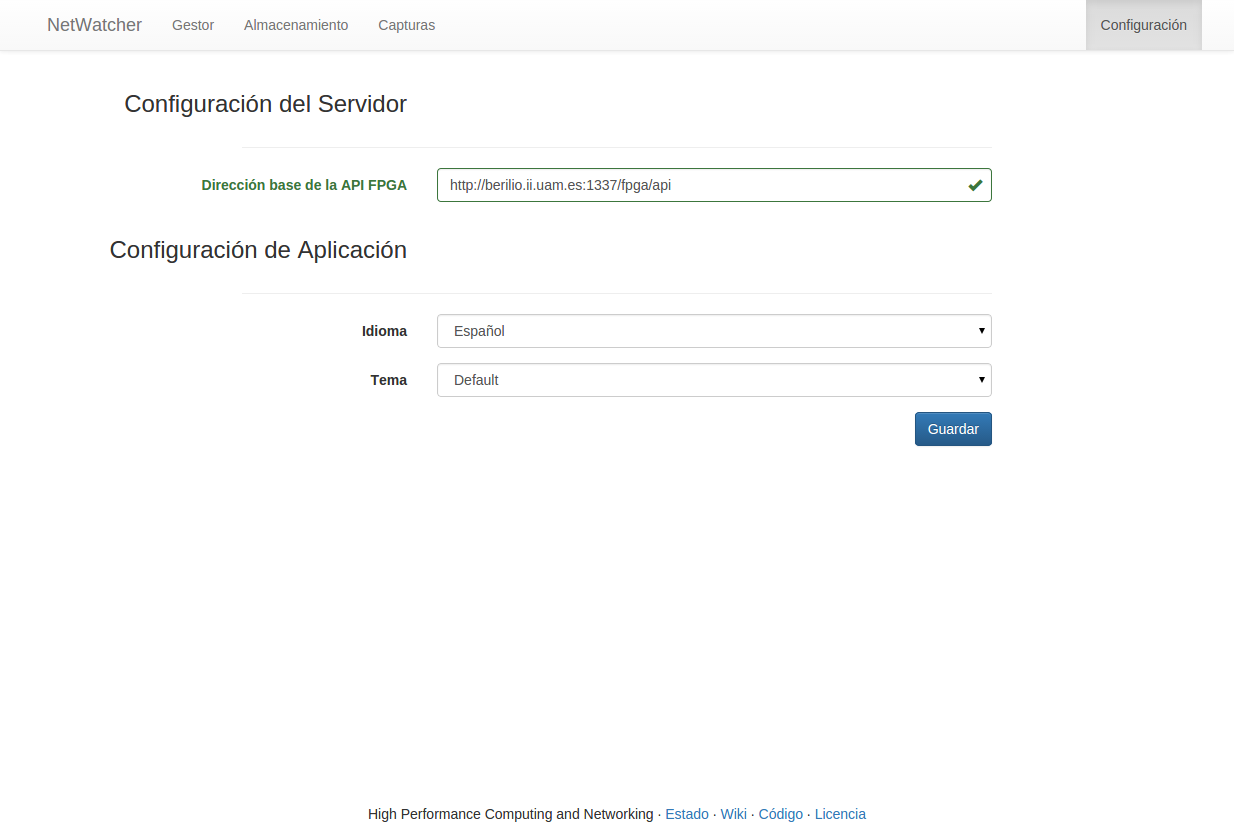
\includegraphics[width=\textwidth,clip=true]{graphics/capturas/configuracion_tema_base}
  \caption{Página de configuración de la interfaz web.}
  \label{fig:captura:configuracion}
\end{figure}


\section{Uso de la aplicación\label{extra:manual:uso}}
Una vez instalado y configurado tanto el \gls{servicioweb} \gls{FPGA} como la interfaz web, todo está listo para utilizar la interfaz. Esta interfaz se puede usar desde cualquier navegador, y tanto en ordenador como en móvil. Todas las pantallas tienen las misma barras de navegación.

Desde la barra de navegación superior se pueden acceder a las siguientes pantallas:
\begin{itemize}
  \item \textbf{Gestor}: administración de la \gls{FPGA}.
  \item \textbf{Almacenamiento}: estadísticas de almacenamiento y del \gls{RAID}, si activo.
  \item \textbf{Capturas}: gestión de las \glspl{traza} almacenadas.
  \item \textbf{Configuración}: explicada en la sección \ref{extra:manual:configweb}.
\end{itemize}

La barra de navegación inferior contiene los siguientes elementos:
\begin{itemize}
  \item \textbf{Estado}: enlace a la pantalla con estado actual del sistema.
  \item \textbf{Wiki}: enlace a la documentación del proyecto.
  \item \textbf{Código}: enlace al repositorio de código del proyecto.
  \item \textbf{Licencia}: despliega la licencia del proyecto.
\end{itemize}

Adicionalmente, se puede acceder a la documentación interna autogenerada del proyecto (en inglés) mediante las siguientes rutas relativas a la dirección base de la interfaz web:
\begin{itemize}
  \item \textbf{Documentación del \gls{servicioweb} \gls{FPGA}}: \texttt{/docs-back-end/}.
  \item \textbf{Documentación de la interfaz web}: \texttt{/docs-front-end/}.
\end{itemize}

En las siguientes subsecciones se explica como utilizar las pantallas de la interfaz web.


\subsection{Gestor\label{extra:manual:gestor}}

TODO: Selección de modo, Figura \ref{fig:captura:gestionseleccion}
\begin{figure}[H]
  \centering
  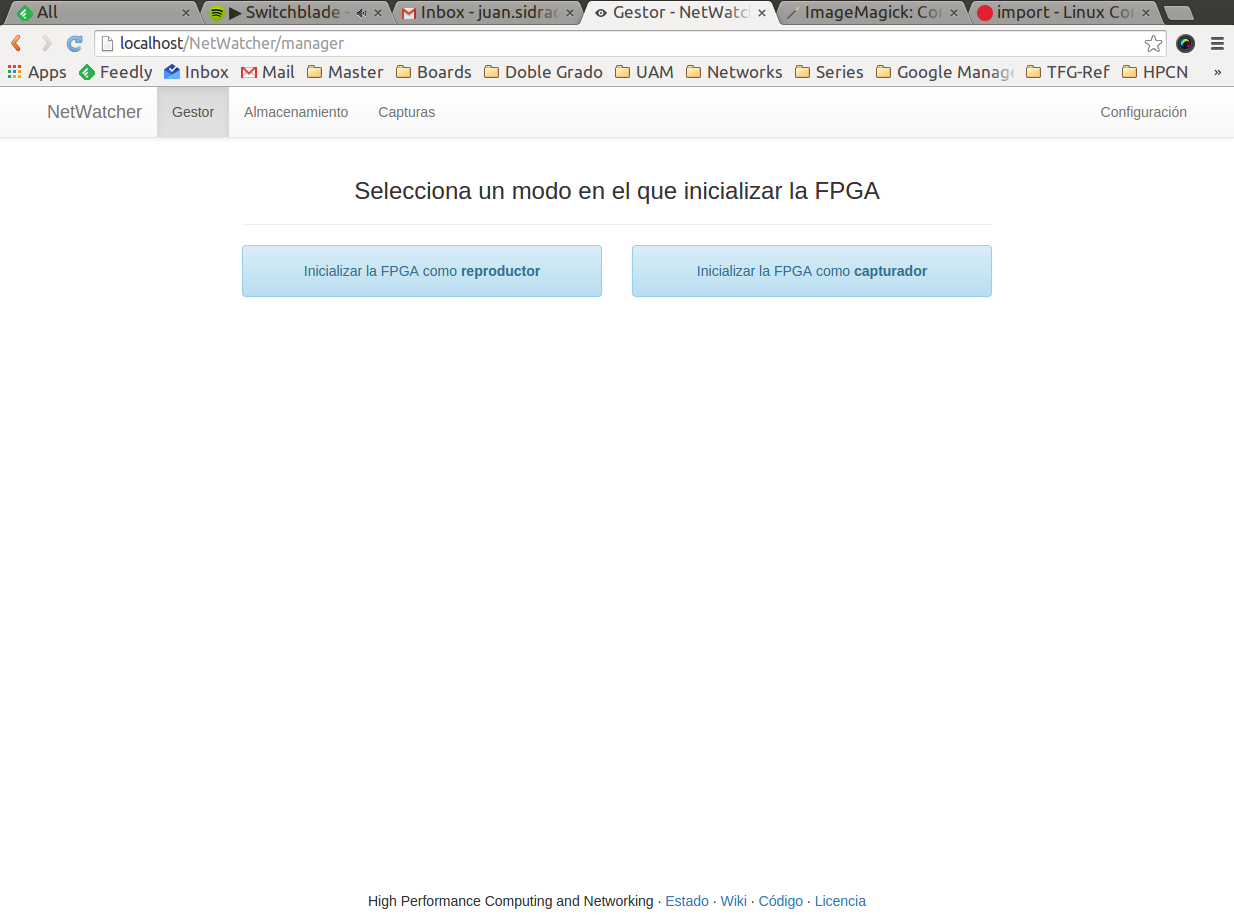
\includegraphics[width=\textwidth,clip=true]{graphics/capturas/gestor_seleccion}
  \caption{Página de gestión - selección de modo.}
  \label{fig:captura:gestionseleccion}
\end{figure}

TODO: Selección de modo en progreso, Figura \ref{fig:captura:gestionprogreso}
\begin{figure}[H]
  \centering
  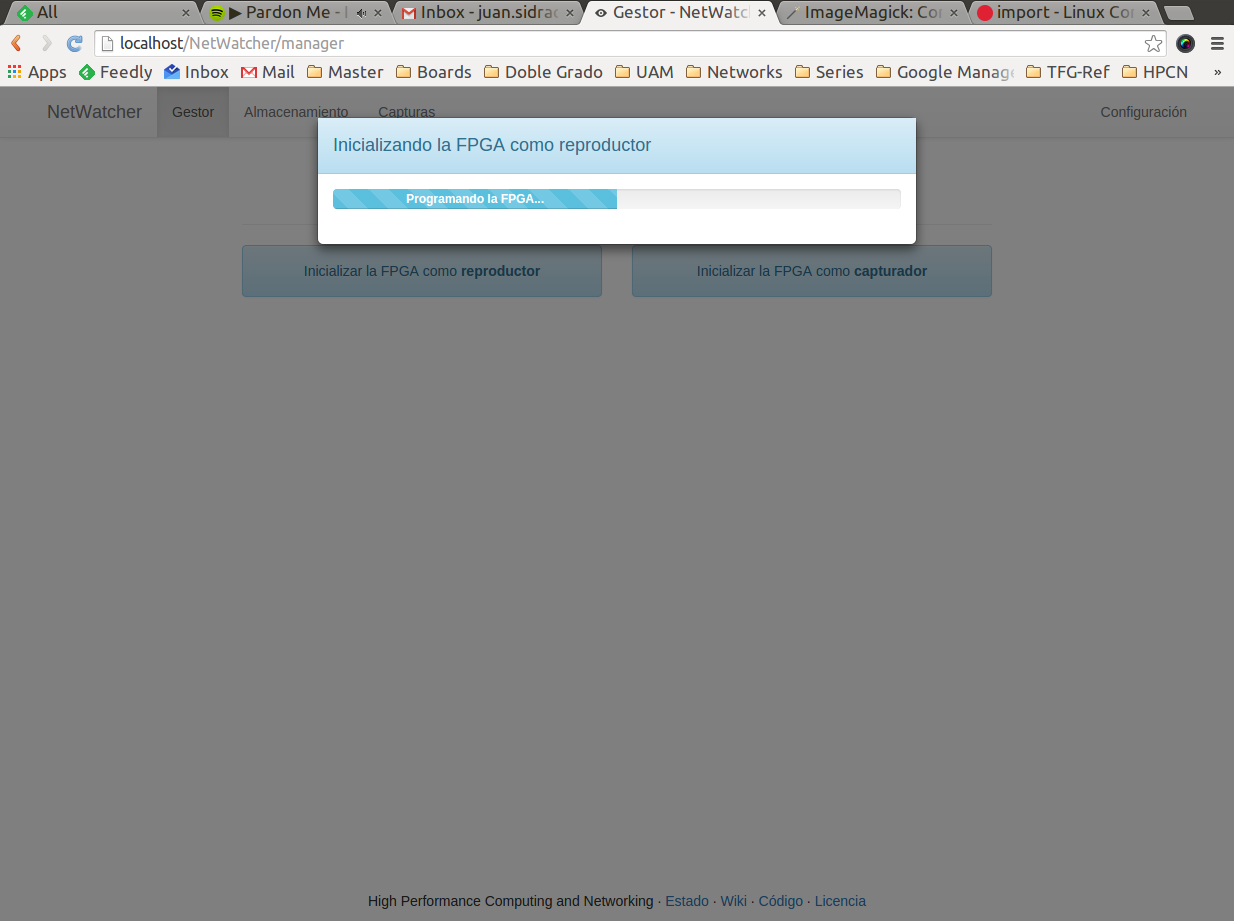
\includegraphics[width=\textwidth,clip=true]{graphics/capturas/gestor_seleccion_progreso}
  \caption{Página de gestión - selección de modo en progreso.}
  \label{fig:captura:gestionprogreso}
\end{figure}

TODO: Capturar tráfico form, Figura \ref{fig:captura:gestioncapturar}
\begin{figure}[H]
  \centering
  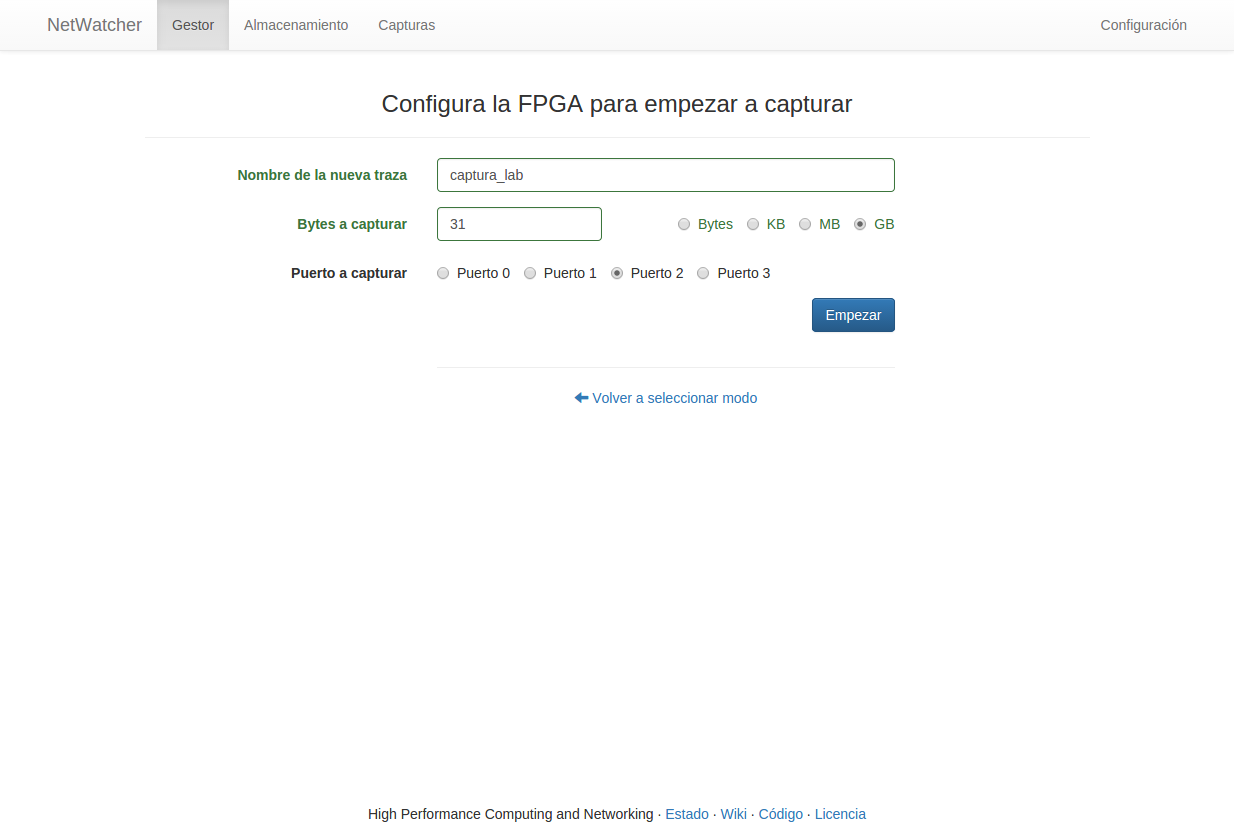
\includegraphics[width=\textwidth,clip=true]{graphics/capturas/gestor_capturar}
  \caption{Página de gestión - capturar tráfico.}
  \label{fig:captura:gestioncapturar}
\end{figure}

TODO: Capturando tráfico, Figura \ref{fig:captura:gestioncapturando}
\begin{figure}[H]
  \centering
  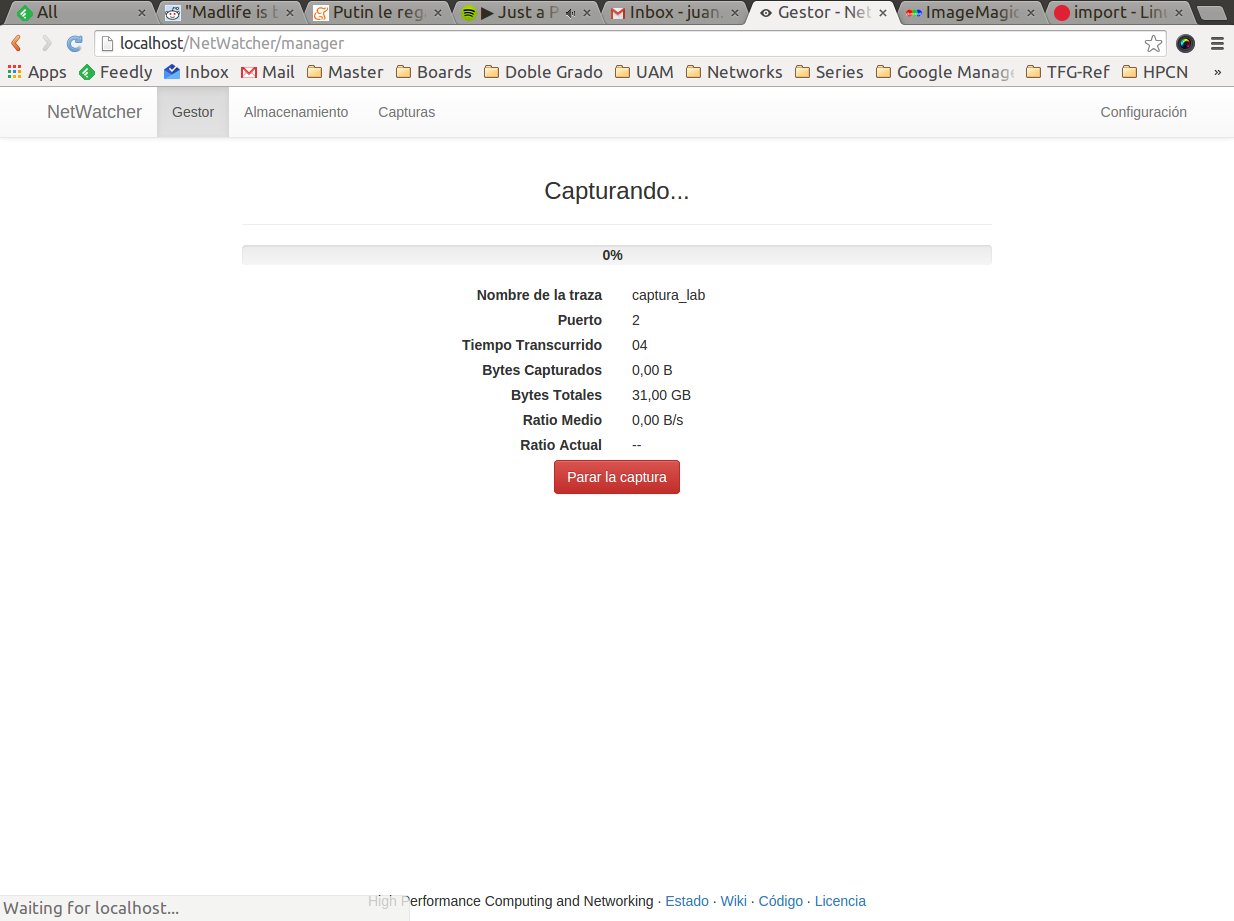
\includegraphics[width=\textwidth,clip=true]{graphics/capturas/gestor_capturando}
  \caption{Página de gestión - capturando tráfico.}
  \label{fig:captura:gestioncapturando}
\end{figure}

TODO: Reproducir traza form, Figura \ref{fig:captura:gestionreproducir}
\begin{figure}[H]
  \centering
  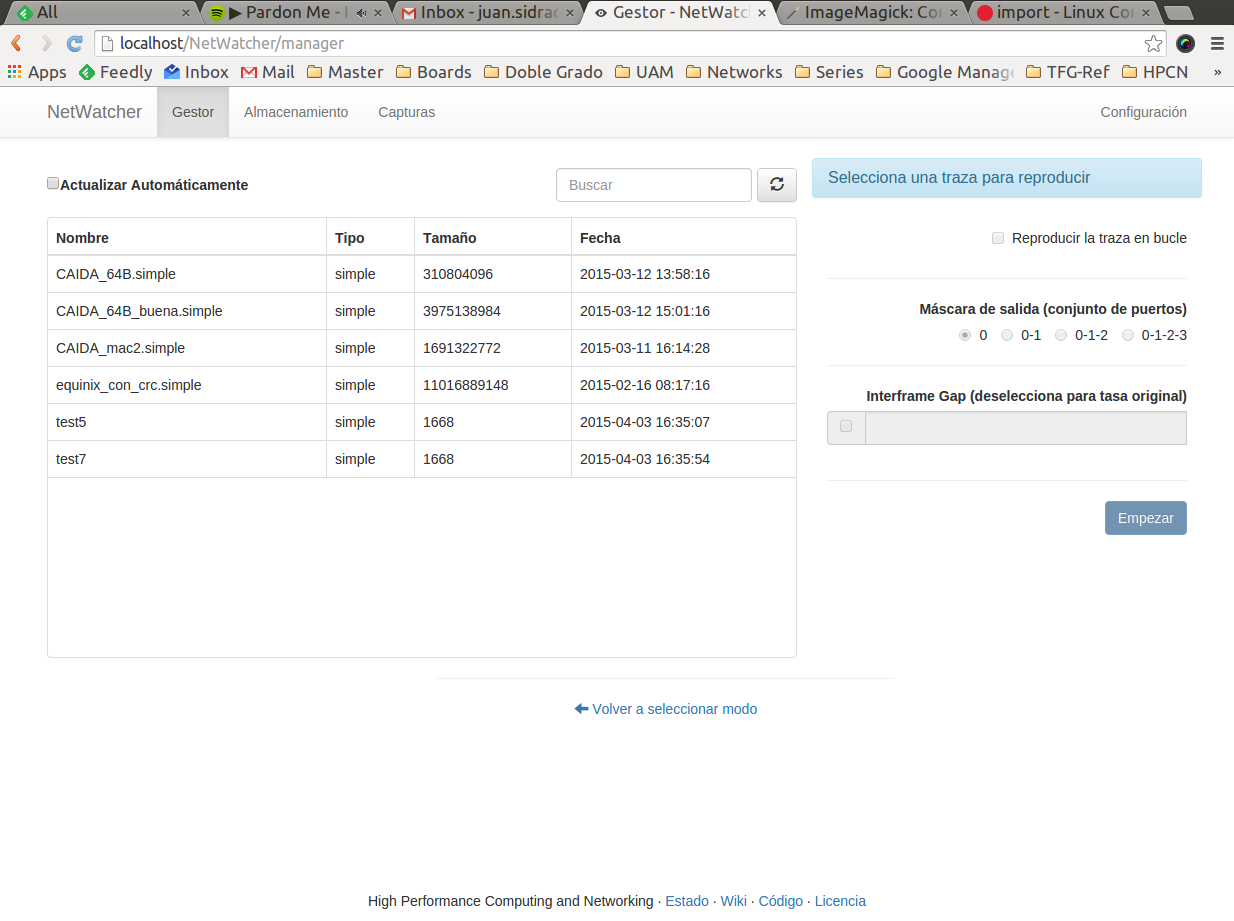
\includegraphics[width=\textwidth,clip=true]{graphics/capturas/gestor_reproducir}
  \caption{Página de gestión - reproducir \gls{traza}.}
  \label{fig:captura:gestionreproducir}
\end{figure}

TODO: Reproduciendo traza, Figura \ref{fig:captura:gestionreproduciendo}
\begin{figure}[H]
  \centering
  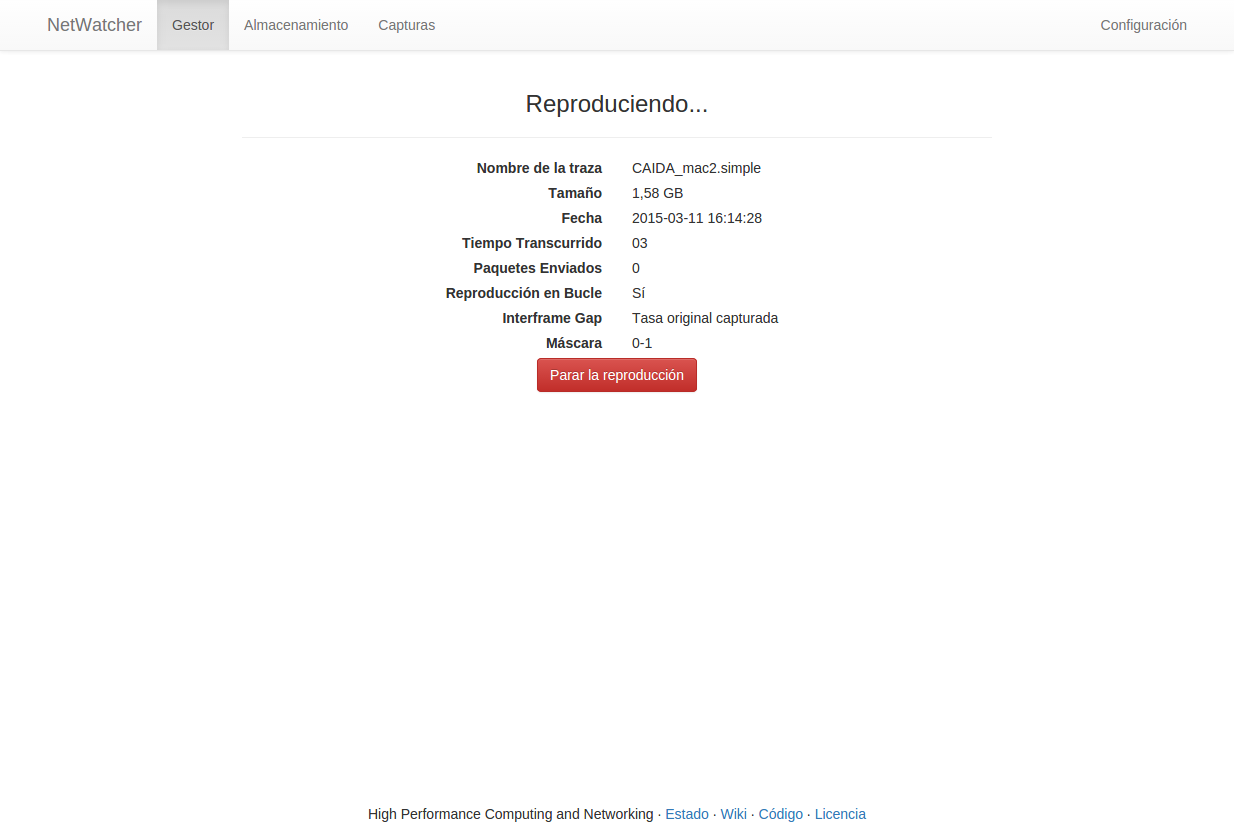
\includegraphics[width=\textwidth,clip=true]{graphics/capturas/gestor_reproduccion}
  \caption{Página de gestión - reproduciendo \gls{traza}.}
  \label{fig:captura:gestionreproduciendo}
\end{figure}


\subsection{Almacenamiento\label{extra:manual:almacenamiento}}
TODO: Estadísticas, formatear raid

TODO: Espacio, Figura \ref{fig:captura:espacio}
\begin{figure}[H]
  \centering
  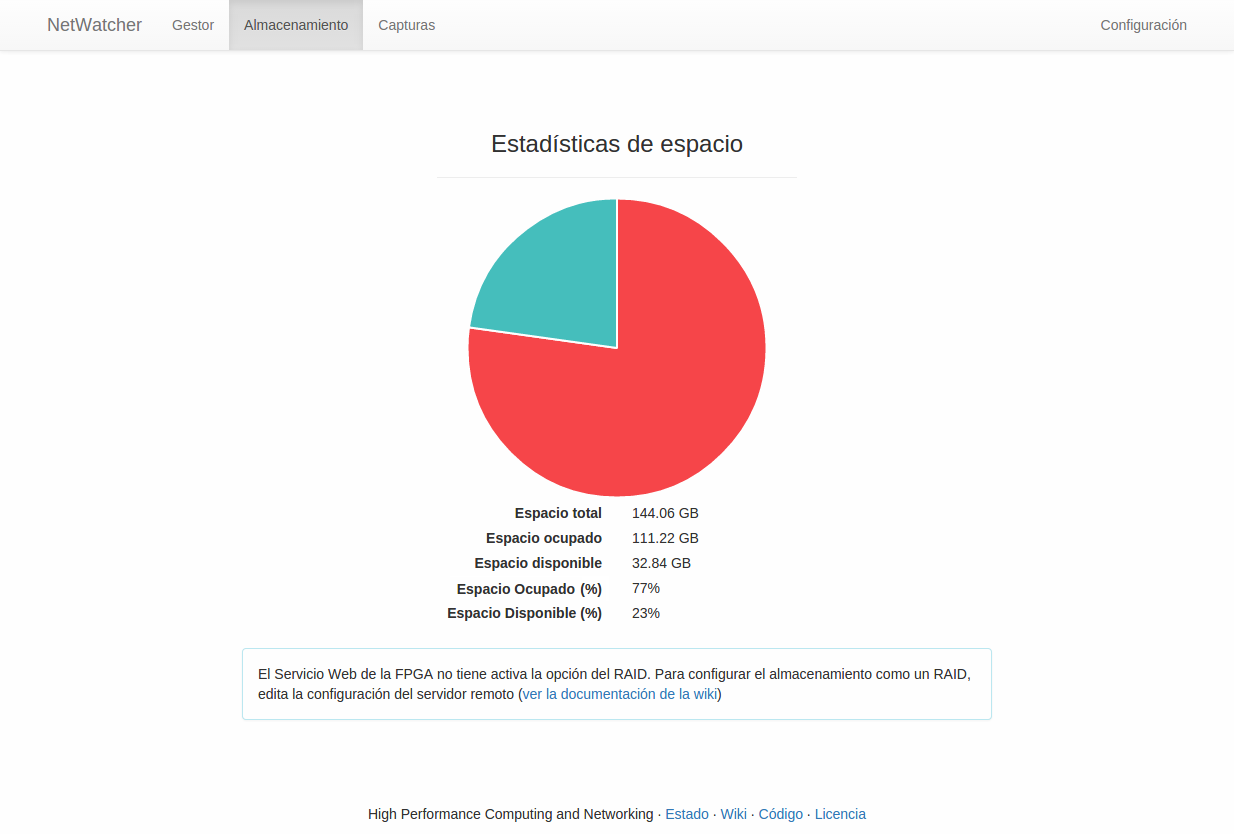
\includegraphics[width=\textwidth,clip=true]{graphics/capturas/almacenamiento_espacio}
  \caption{Página de almacenamiento, con \gls{RAID} no activo.}
  \label{fig:captura:espacio}
\end{figure}

TODO: RAID, Figura \ref{fig:captura:raid}
\begin{figure}[H]
  \centering
  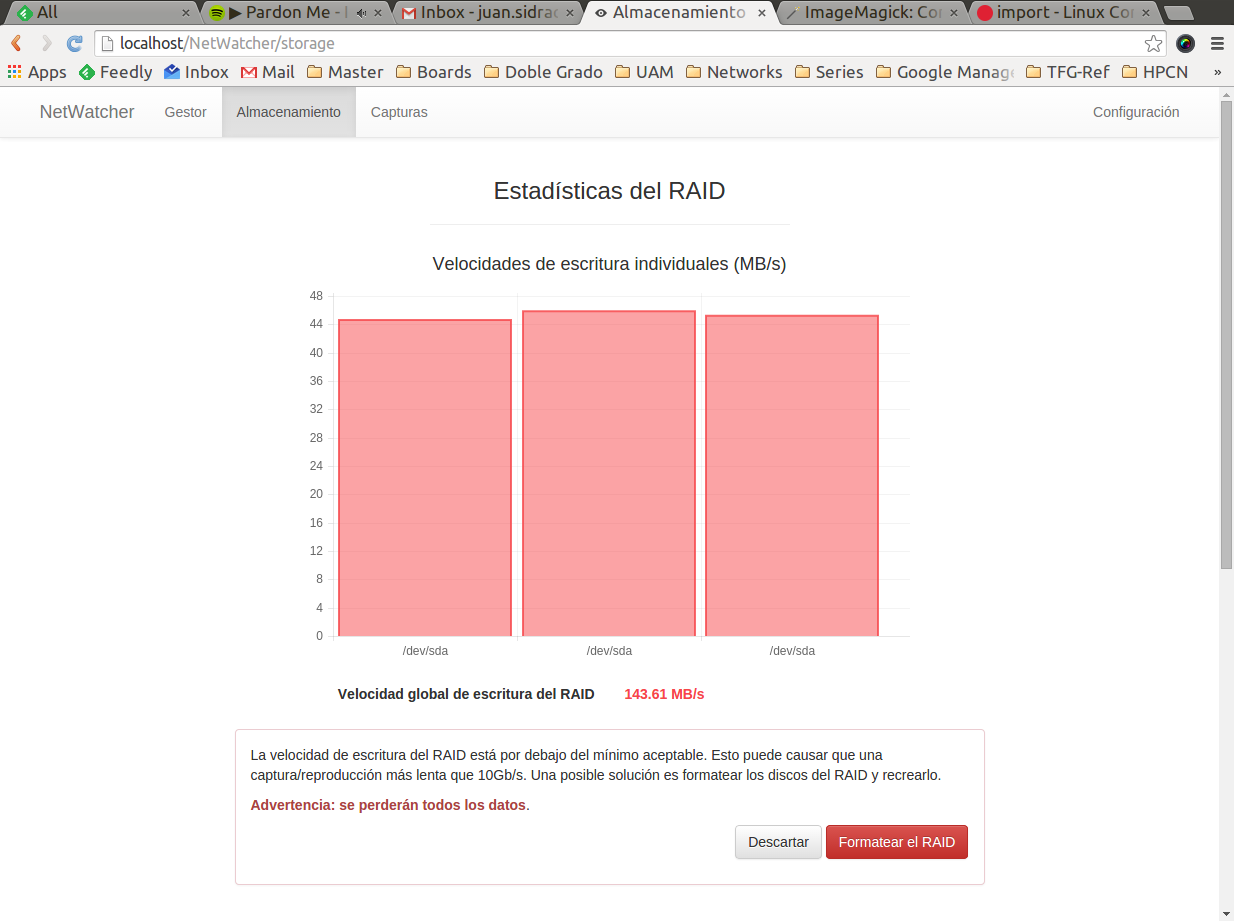
\includegraphics[width=\textwidth,clip=true]{graphics/capturas/almacenamiento_raid}
  \caption{Página de almacenamiento, con \gls{RAID} activo.}
  \label{fig:captura:raid}
\end{figure}


\subsection{Capturas\label{extra:manual:capturas}}

TODO: Renombrar, convertir <->, borrar, Figura \ref{fig:captura:capturas}
\begin{figure}[H]
  \centering
  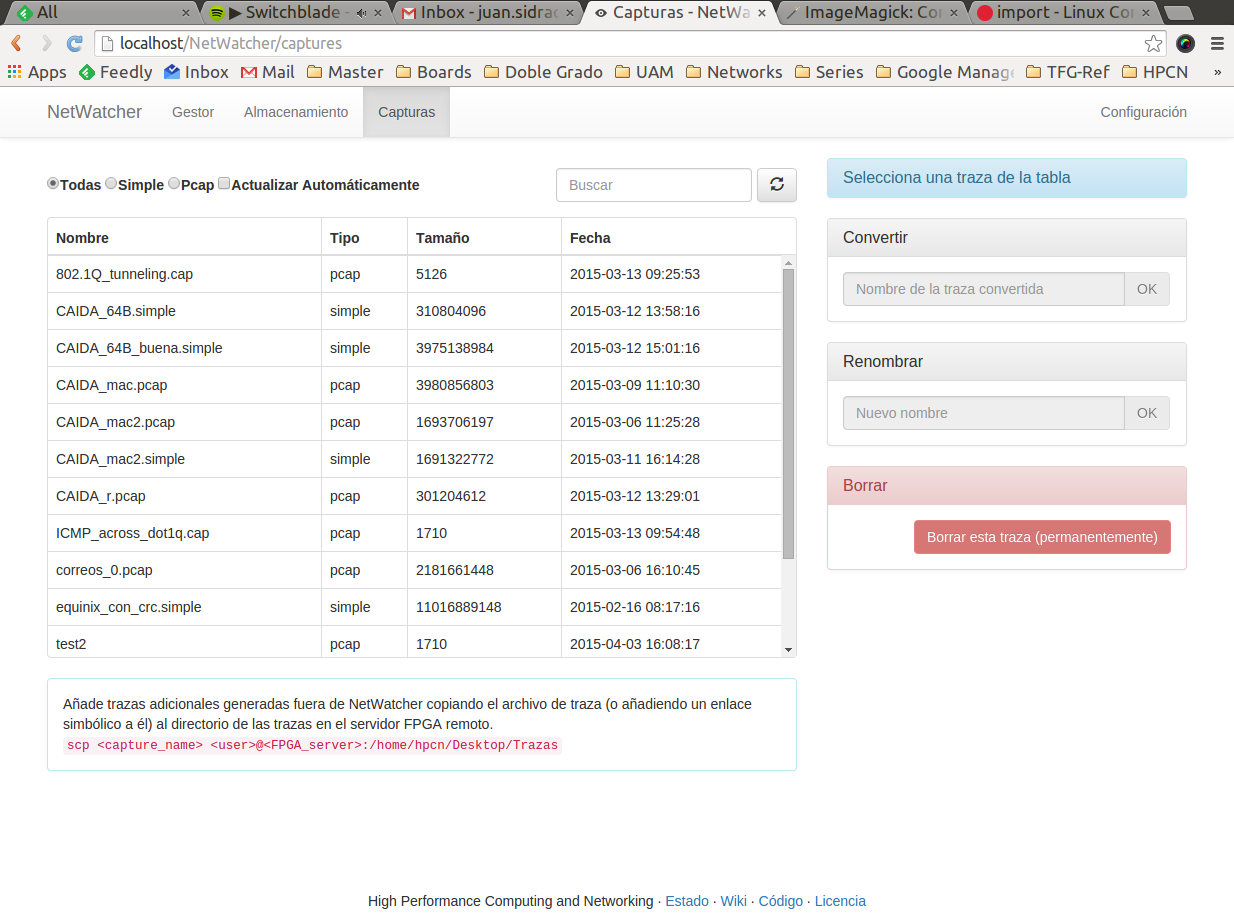
\includegraphics[width=\textwidth,clip=true]{graphics/capturas/capturas}
  \caption{Página de capturas.}
  \label{fig:captura:capturas}
\end{figure}


\subsection{Estado\label{extra:manual:estado}}

TODO: Estado, Figura \ref{fig:captura:estado}
\begin{figure}[H]
  \centering
  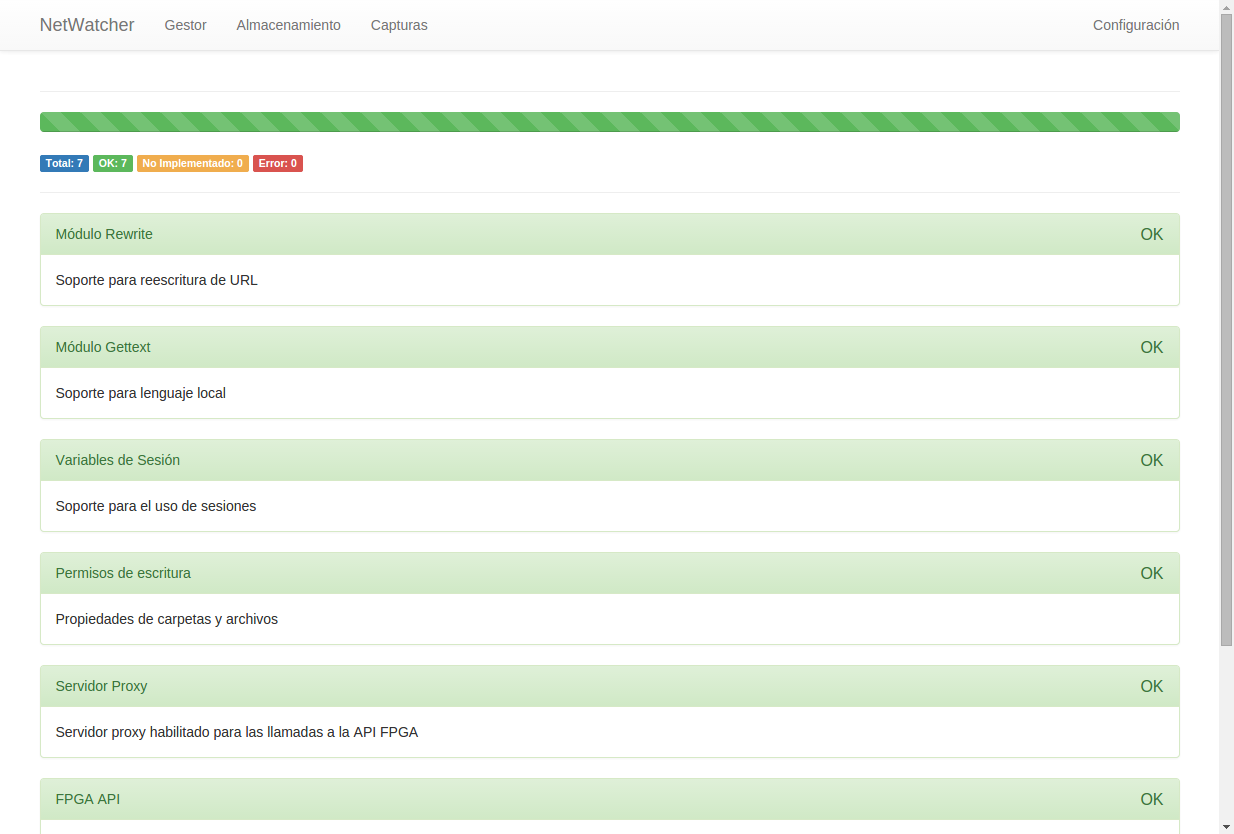
\includegraphics[width=\textwidth,clip=true]{graphics/capturas/estado}
  \caption{Página de estado del sistema.}
  \label{fig:captura:estado}
\end{figure}


\section{Solución de problemas\label{extra:manual:solucion}}

Si tras seguir las instrucciones paso a paso algo impide el correcto funcionamiento de la aplicación, puedes consultar la página de solución de problemas (en inglés), disponible dentro del repositorio del proyecto en:

\href{https://github.com/JSidrach/NetWatcher/blob/master/docs/wiki/Troubleshooting.md}{github.com/JSidrach/NetWatcher/blob/master/docs/wiki/Troubleshooting.md}